\documentclass{article}
\usepackage[T1]{fontenc}
\usepackage[utf8]{inputenc}
\usepackage{listings}
\usepackage{color}
\definecolor{red}{rgb}{0.6,0,0} % for strings
\definecolor{green}{rgb}{0.25,0.5,0.35} % comments
\definecolor{purple}{rgb}{0.5,0,0.35} % keywords
\definecolor{docblue}{rgb}{0.25,0.35,0.75} % javadoc
 
\lstset{
	basicstyle=\normalsize\ttfamily,
	keywordstyle=\color{purple}\bfseries,
	stringstyle=\color{red},
	commentstyle=\color{green},
	morecomment=[s][\color{docblue}]{/**}{*/},
	tabsize=4,
	showspaces=false,
	showstringspaces=false
}
	
\usepackage{graphicx}
\usepackage{fancyhdr}
\usepackage[margin=1.2in]{geometry}
\geometry{a4paper, left=20mm, right=20mm, top=20mm, bottom=20mm}
\linespread{1.5}
\begin{document}

\begin{titlepage}
	\begin{center}
		{\LARGE College of Engineering, Trivandrum}\\[3cm]
		\linespread{1.2}\huge {\bfseries Microprocessor Lab}\\[3cm]
		\linespread{1}
		
\includegraphics[width=8cm]{img/emblem.jpeg}\\[1cm]
		{\Large Gokul K\\ S6 CSE \\ Roll No: 21\\ TVE18CS021 }\\[1cm]
		\textit{ }\\[1cm]
		{\LARGE 
			Department of Computer Science\\[0.2cm]
			\today 
		}
	\end{center}
	
\end{titlepage}
\large

\newpage
\setlength{\headheight}{15.2pt}
\pagestyle{fancy}
\fancyhf{}
\fancyhead[RO]{\fontsize{12}{12}\selectfont\nouppercase\leftmark} 
\fancyhead[LO]{\fontsize{9}{12}\selectfont\nouppercase\rightmark} 

% Use the current experiment file from experiments/ folder
\section{16 bit addition}
\subsection{Aim}
To add two 16 bit numbers

\subsection{Code}
\begin{lstlisting}
ORG 0000H

; ROR1 forms 2000H
MOV R0, #20H
MOV R1, #00H

; R2R3 forms 3000H
MOV R2, #30H
MOV R3, #00H

; Addition of lower byte
MOV A, R1
ADD A, R3
MOV R5, A ; Lower byte of result stored in R5

; Addition of upper byte
MOV A, R0
ADDC A, R2
MOV R4, A ; Upper byte of result stored in R4

END
\end{lstlisting}

\subsection{Output}
\textbf{Input} 2000H (R0R1), 3000H (R2R3)\\
\textbf{Output} 5000H (R4R5)
\begin{center}
	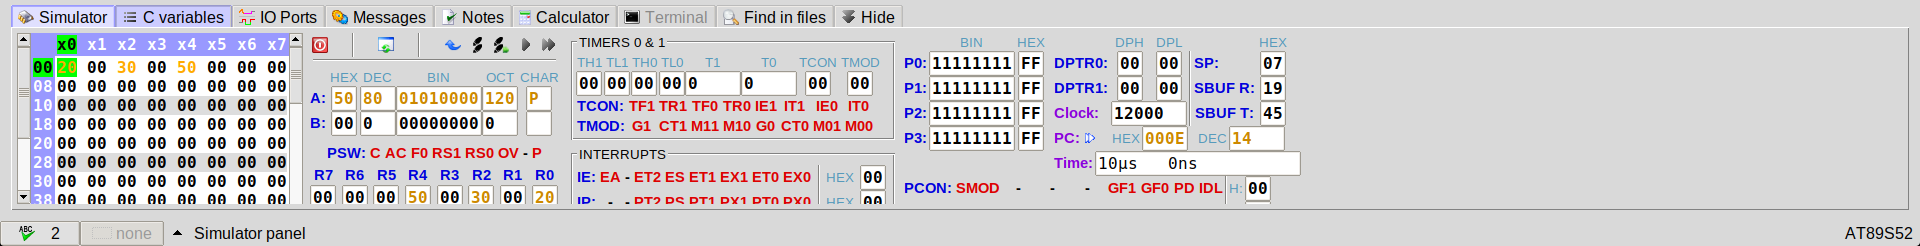
\includegraphics[width=\textwidth]{img/p21.png}
\end{center}

\subsection{Result}
Two 16 bit numbers were added in mcu8051ide



\newpage
\section{16 bit substraction}
\subsection{Aim}
To substract two 16 bit numbers

\subsection{Code}
\begin{lstlisting}
ORG 0000H

; R0R1 forms 2000H
MOV R0, #20H
MOV R1, #00H

; R2R3 form 1000H
MOV R2, #10H
MOV R3, #00H

; Substraction of upper bytes
MOV A, R0
SUBB A, R2
MOV R4, A ; Upper byte of result stored in R4

; Substraction of lower bytes
MOV A, R1
SUBB A, R3
MOV R5, A ; Upper byte of result stored in R5

END
\end{lstlisting}

\subsection{Output}
\textbf{Input} 2000H (R0R1), 1000H (R2R3)\\
\textbf{Output} 1000H (R4R5)
\begin{center}
	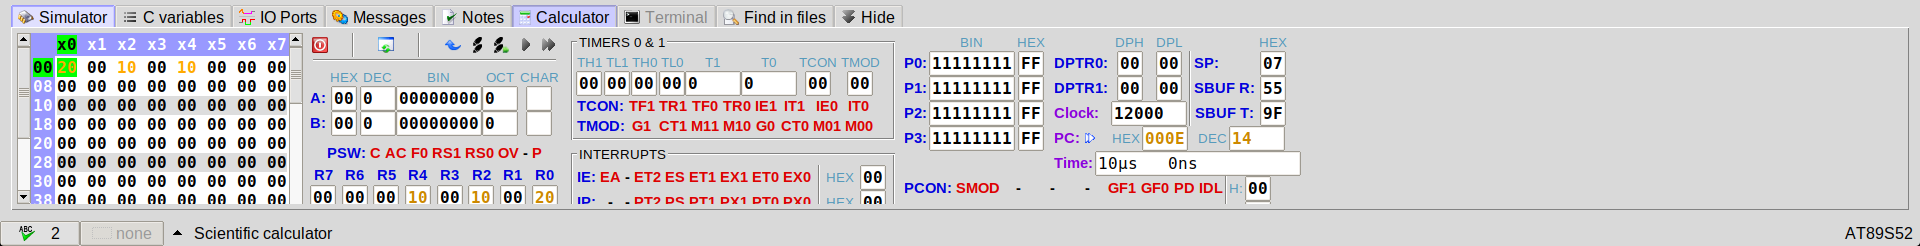
\includegraphics[width=\textwidth]{img/p22.png}
\end{center}

\subsection{Result}
Two 16 bit numbers were substracted in mcu8051ide



\newpage
\section{8 bit multiplication \& division}
\subsection{Aim}
To multiply and divide two 8bit numbers

\subsection{Code}
\begin{lstlisting}
ORG 0000

; Multiplying 20H with 10H
MOV A, #20H
MOV B, #10H
MUL AB
MOV R0, B ; Storing upper byte of result
MOV R1, A ; Storing lower byte of result

; Dividing 20H with 10H
MOV A, #20H
MOV B, #10H
DIV AB
MOV R2, B ; Remainder of division
MOV R3, A ; Quotient of division	

END
\end{lstlisting}

\subsection{Output}
\textbf{Input} 20H (R0R1), 10H (R2R3)\\
\textbf{Output}\\
Multiplication: 0200H (R0R1)\\
Division: Remainder - 00 (R2), Quotient - 02H (R3)
\begin{center}
	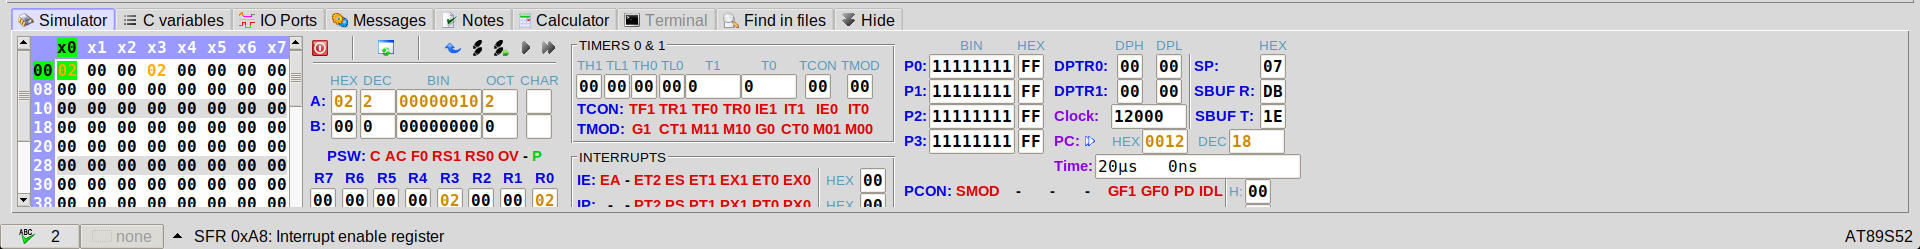
\includegraphics[width=\textwidth]{img/p23.png}
\end{center}

\subsection{Result}
Two 8 bit numbers were multiplied and divided in mcu8051ide

\end{document}